\documentclass{article}
\usepackage[margin=3cm]{geometry}
\usepackage{amssymb}

% Figures
\usepackage{graphicx}
\usepackage{color}

% Page formatting
\newsavebox{\notetitle}
\newsavebox{\noteauthor}
\newsavebox{\notenumber}
\newsavebox{\notedate}
\renewcommand{\title}[1]{\sbox{\notetitle}{\Large{\textbf{#1}}}}
\renewcommand{\author}[1]{\renewcommand{\and}{\quad}\sbox{\noteauthor}{\large{#1}}}
\renewcommand{\date}[1]{\sbox{\notedate}{\large{#1}}}
\newcommand{\nb}[1]{\sbox{\notenumber}{\Large{\textbf{#1}}}}
\newcommand{\makemadtitle}{
  \hrule
  \vspace{.5em}
  \noindent
  \begin{center}
  \textbf{
  {\centering
\includegraphics[height=3cm]{logoCHISTERA2014}}\\
   {\centering\Large COACHES project, CHIST-ERA 2014 program}
  }
  \end{center}
  \vspace{.5em}
 
  \hrule
  \vspace{3em}
  \begin{center}
    \begin{large}\textbf{ Note~\usebox{\notenumber}.}\end{large}\\[.5em]
    \begin{Large}\textbf{\usebox{\notetitle}}\end{Large}\\[2em]
    \begin{large}\usebox{\noteauthor} --- \usebox{\notedate}\end{large}
  \end{center}
  \vspace{3em}
}

% Various macros and environments
\newtheorem{prop}{Proposition}
\newtheorem{proposition}[prop]{Proposition}
\newtheorem{defn}{Definition}
\newtheorem{definition}[defn]{Definition}
\newtheorem{cor}{Corollary}
\newtheorem{corollary}[cor]{Corollary}
\newtheorem{exmp}{Example}
\newtheorem{example}[exmp]{Example}
\newtheorem{lem}{Lemma}
\newtheorem{lemma}[lem]{Lemma}
\newtheorem{fact}{Fact}
\newtheorem{thm}{Theorem}
\newtheorem{theorem}[thm]{Theorem}
\newtheorem{prob}{Problem}
\newtheorem{problem}[prob]{Problem}
\newtheorem{rem}{Remark}
\newtheorem{remark}[rem]{Remark}
\newtheorem{conj}{Conjecture}
\newtheorem{conjecture}[conj]{Conjecture}
\newenvironment{pf}{{\bf Proof }}{\hfill$\Box$\par}
\newenvironment{proof}{{\bf Proof }}{\hfill$\Box$\par}
\newcommand{\spaceafterproof}{\vspace{1em}}

% NOTE ITSELF BELOW %%%%%%%%%%%%%%%%%%%%%%%%%%%%%%%%%%%%%%%%%%%%%

\title{ Semantic map and event-based reasoning}
\author{COACHES Consortium: Abdel-Illah, Luca, Esra}
\nb{: Draft WP1 }

\date{\today}

\begin{document}

\includegraphics[height=2cm]{logoUNICAEN}

\includegraphics[height=2cm]{logoSapienza.png}
\includegraphics[height=2cm]{logo-vub}

\includegraphics[height=2cm]{logoSebanci}


\makemadtitle

\vspace*{1.0in}
\begin{abstract}
 This document describes the general principles of the Knowledge-based reasoning developed in WP1 where representation of the semantic map, spatial information, and events is described and the commonsense reasoning technique is presented. 
  \end{abstract}

\vspace*{1.5in}

\fbox{
\begin{minipage}{1.0\textwidth}
\begin{center}
 $\copyright$, THE COACHES CONSORTIUM \\
The copyright in this document is the property of the COACHES Consortium. This document is supplied by the COACHES consortium on the express terms that it is to be treated as confidential. This document is not external distribution without the project manager's permission. 
\end{center}
\end{minipage}
}
\newpage
\section{Introduction}
This document consists of describing different principles of the Knowledge-based reasoning module developed in WP1. This  module receives different information from different units, sensor or other modules of the architecture particularly the multi-modale interface and perception modules. This information concerns the semantic map, spatial information and human activities. From these information, the reasoning module should infer new goals to accomplish. This list of goals is sent the decision module computing the behavior policy of the robot to accomplish goals and sent it the exception module using Petri-Net plan execution. The general principle is depicted in Figure \ref{WP1principle}.
\begin{figure}[htbp]
\begin{center}
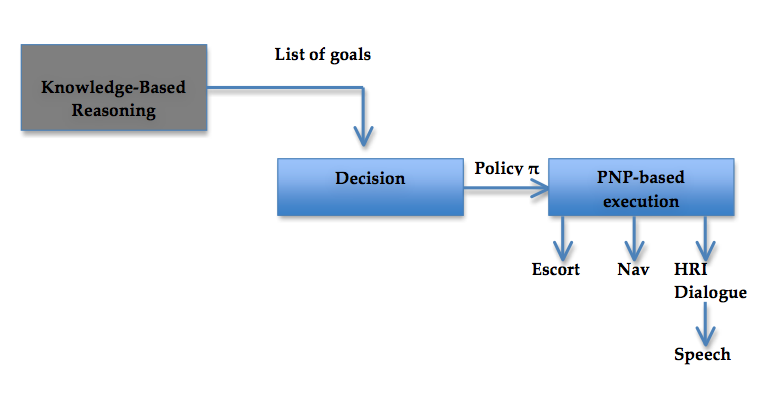
\includegraphics[height=10cm]{WP1Principles}
\caption{General principles of interaction between KB  and decision modules}
\label{WP1principle}
\end{center}
\end{figure}

\section {Representation and reasoning}
In this section we present the main concepts we will consider to detect events in the environnement due to external units or human activities. To this end, we consider the semantic map, spatial information and human activities 
\subsection {Semantic map}
For the mall map, we consider different type of areas: restaurant, rest, WC, caf�, shops, halls, corridors, offices and doors. For shops, services and restaurants we consider different categories:
\begin{itemize}
\item {\it Shop categories}: dress shop , women dress shop, kid dress shop, men dress shop, makeup store, store perfume, sport store,
\item {\it Restaurant categories}: French, Japanese, Chinese, Italian, Oriental, African, fastfood, .. 
\item {\it Service categories}: security, information, healthcare
\end{itemize}
Other areas and categories could be considered according to the use case requirements.
For all areas, we have to define their localisation using local or global position using local map or GPS.
To this end, we introduce different predicates: type, category and position
\subsection{Type predicate}
{\tt\bf type}(id, door $\|$ shop $\|$ restaurant $\|$ service $\|$ caf� $\|$ corridor $\|$ rest $\|$ wc)

\paragraph*{\bf Example}~\\

{\tt\bf type}(McDonald, restaurant); 

{\tt\bf type}(main\_entrance\_ouest\_1, door); 

{\tt\bf type}(hall\_rive\_marin, hall).

\subsection{Category predicate}
{\tt\bf category}(shop\_id, kid\_dress $\|$ men\_dress$\|$woman\_dress $\|$ dress $\|$ sport $\|$ perfume $\|$ decoration)\\
{\tt\bf category}(restaurant\_id, fastfood $\|$Italian$\|$French $\|$Chinese $\|$Japenese $\|$ Orient)\\
{\tt\bf category}(service\_id, Security$\|$information $\|$ healtcare)\\

\paragraph*{\bf Example}~\\
type(HM\_id, shop) ; category(HM\_id, dress) 
type(macdonald, restaurant) ;  category(macdonald, fastfood)\\

\subsection{Areas status predicate}
\begin{itemize}
\item {\tt\bf Isopen} \\
{\tt\bf Isopen}(id\_door, true$\|$false): meaning that the door is open or not.\\
{\tt\bf Isopen}(id\_hall, true) meaning that the robot can navigate in this hall\\
\item {\tt\bf Connect} \\
 {\bf\tt Connect} (id\_door; area1, area2), for example connect(door\_hm, HM\_id,
hall\_rive\_marine) meaning that door\_hm connects the shop HM to the hall Rive
marine of the mall.
\item {\tt\bf Position} \\
 {\tt\bf Position}(id\_area, local$\|$GPS, coordinates)
 \end{itemize}

\subsection{Spatial relations}
In this section we consider all spatial relations and information:
\begin{itemize}
\item {\tt\bf Infrontof}(person\_id, area\_id)
\item {\tt\bf Nearby}(person\_id, area\_id)
\item {\tt\bf At}(person\_id, location)
\item {\tt\bf In}(person\_id $\|$ object\_id, areas\_id)
 \end{itemize}
\subsection{Human activities}
\begin{itemize}
\item {\tt\bf Motionless}(person\_id, time\_t, location)
\item {\tt\bf Request} (request\_id,request\_type, person\_id, location\_t) where {\it Request\_type}  could be escorting\_to(location),informing\_about(area\_id), guiding\_to(location)
\item {\tt\bf Rest\_Area} (person\_id, time\_t, location)
 \end{itemize}
  \subsection{Commonsense and event-based Reasoning}
  \subsubsection{Event Definition}
  \begin{defn}
  An {\bf Event} is a tuple defined by the actor of the event, where the event has been occurred, when and what is the semantic of the event described by spatio-temporal relations or human activities. 
  \[ Event = <actor, location, time, semantic> \] 
  where semantic = At $\|$ In $\|$ Infrontof $\|$ motionless $\|$ rest\_area $\|$ request \\
  \end{defn}
   \subsubsection{Event-based reasoning and goal generation}
   From the list of predicates and events, we create a list of goals to send to the decision module. In the following these are some commonsense rules to generate goals. 
   \begin{itemize}
\item  {\bf joint escorting goal generation}: \\
  If request\_type=escorting\_to(location) and in(location,hall\_id1) and in(robot, hall\_id2) and hall\_id1 $\neq$ hall\_id2 then \\
  add(list\_goal, create\_task (task\_id joint\_escorting\_task, hall\_id2, hall\_id1, location))
\item  {\bf Surveillance goal generation} \\
  If event(object\_id,location,time\_t,in(object\_id,hall\_id)) then \\
  add(list\_goal, create\_task(task\_id, surveillance\_task, location, object\_id))
\item {\bf Advertising goal generation} \\
   If event(person\_id,location,time\_t,infrontof(person\_id, shop\_id) then \\
   add(list\_goal, create\_task(task\_id, advertising\_task, location, person\_id, shop\_id)
\item $\dots$
   \end{itemize}
   
  \section{Conclusion}
  
  This draft describes in an abstract way what we can expect to have in the KB module. Many concepts should be defined and deepened to provide an effective reasoning module. Representation and reasoning techniques should be discussed. Many commonsense reasoning rules should be defined, spatial reasoning and computation of spatial relations from robot and people locations have to be defined. This could also be discussed in the next phone meeting.
     
\end{document}
